Figure~\ref{fig:4:fw} in Chapter~\ref{chap:cc.fw} shows the structure of the
congestion control framework described in this thesis. The framework
categorizes \emph{In-path} and \emph{Out-of-path} sources and
\emph{out-of-band} signaling for implementing congestion control, which are
discussed in this chapter. This chapter is based on our work on congestion
control for interactive multimedia applications, which is documented in
\citepub{c:3grc}, \citepub{c:glass}.

In \citepub{c:3grc}, when the available link capacity changes at a routers (in
this case, the 3G base stations), it notifies the endpoint connected to it
about the current capacity. Based on the notifications the sender adapts the
sending rate of the video call.

In \citepub{c:glass}, we explore the use of coverage maps for congestion
control. The map server collect throughput information from the mobile
clients, which also add geo-location information along with the throughput
information. This assists the map server to build a bandwidth and coverage map
and is queried by the mobile to predict coverage outage.

\section{In-path Congestion Cues}

In some network deployments, routers along the media path are capable of
detecting congestion before the queue overflows, typically, using active queue
management (e.g., RED). A router marks a packet, indicating that the packet
experienced congestion and the router would soon drop packets for this
flow~\cite{rfc3168}. The receiver on receiving this indication keeps a counter
for the number of ECN marked IP packets and signals it to the sender. For
performing congestion control, the sender typically treats the count of ECN
marked packets as lost packets~\cite{rfc6679}. For example, the sender uses
the sum of the reported loss events and the reported ECN events as the
\emph{p} (loss) value in the TFRC equation. Network-Assisted Dynamic
Adaptation (NADA)~\cite{rmcat-nada} propose a delay-based congestion control,
the receiver measures congestion by aggregating the packet loss count,
reported ECN markings, and one-way delay measurements into a single cue. The
sender calculates the new rate based on the variation in the delay cue
compared to earlier measurements and the priority of the multimedia
stream~\cite{pv-nada}.


In \citepub{c:3grc}, we implement a network-assisted congestion control
scheme, wherein, base-stations connected to the mobile clients notify them
about the available capacity. In wireless networks, such as 3G/LTE, the last
hop is typically the bottleneck because the core network is well 

% ECN, PCN, BW indication


\begin{figure}
  \centerline{
    \subfloat{
      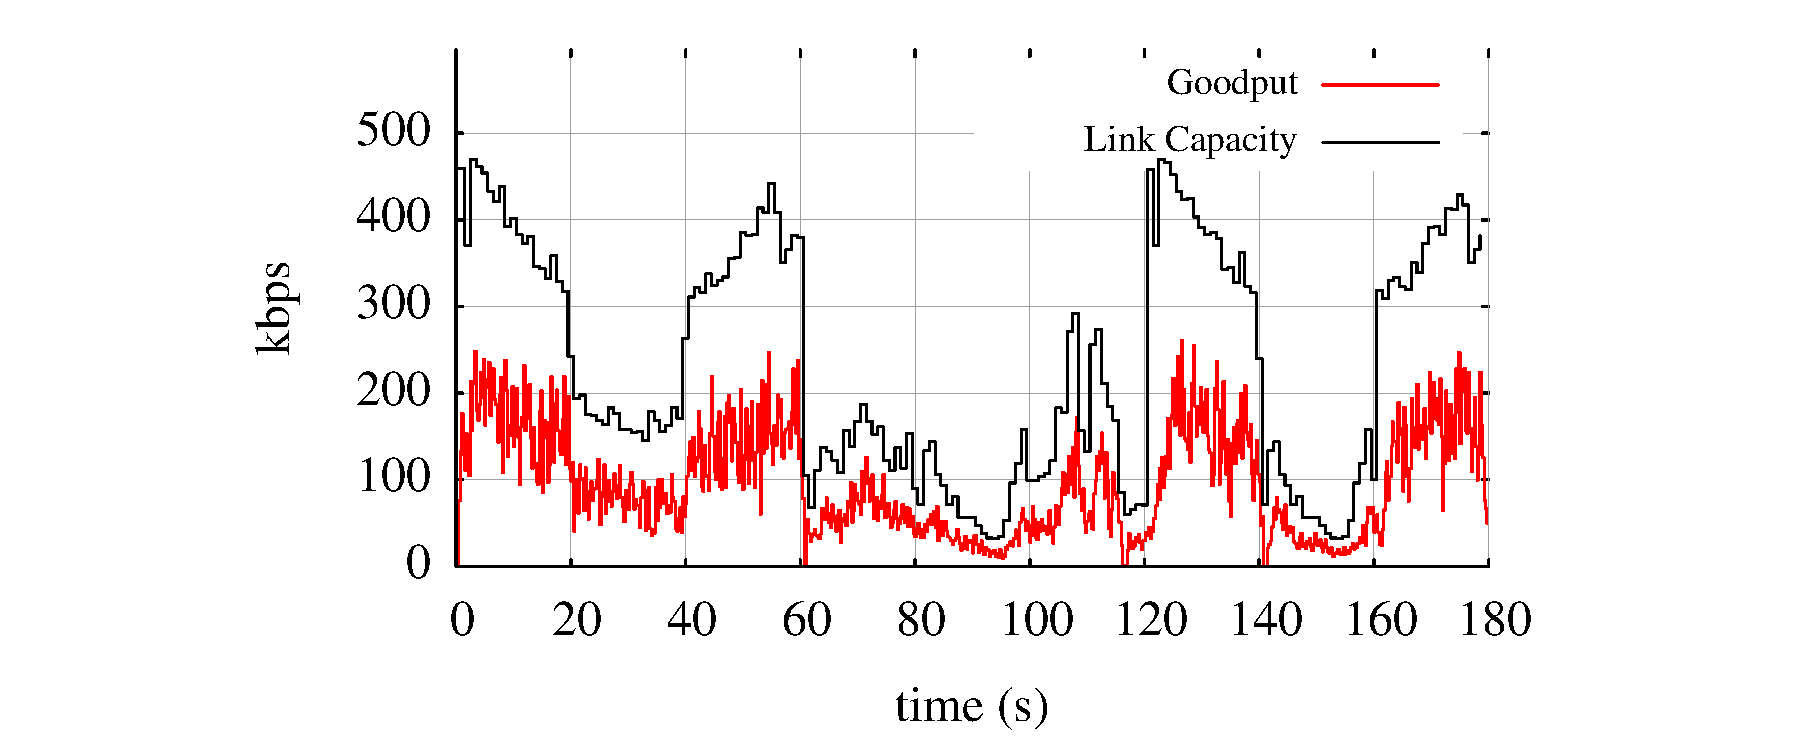
\includegraphics[width=0.5\textwidth, clip=true, trim=3cm 0 4.5cm 0]
      {chap8_graph_3g_tmmbr_a}
    }
    \subfloat{
      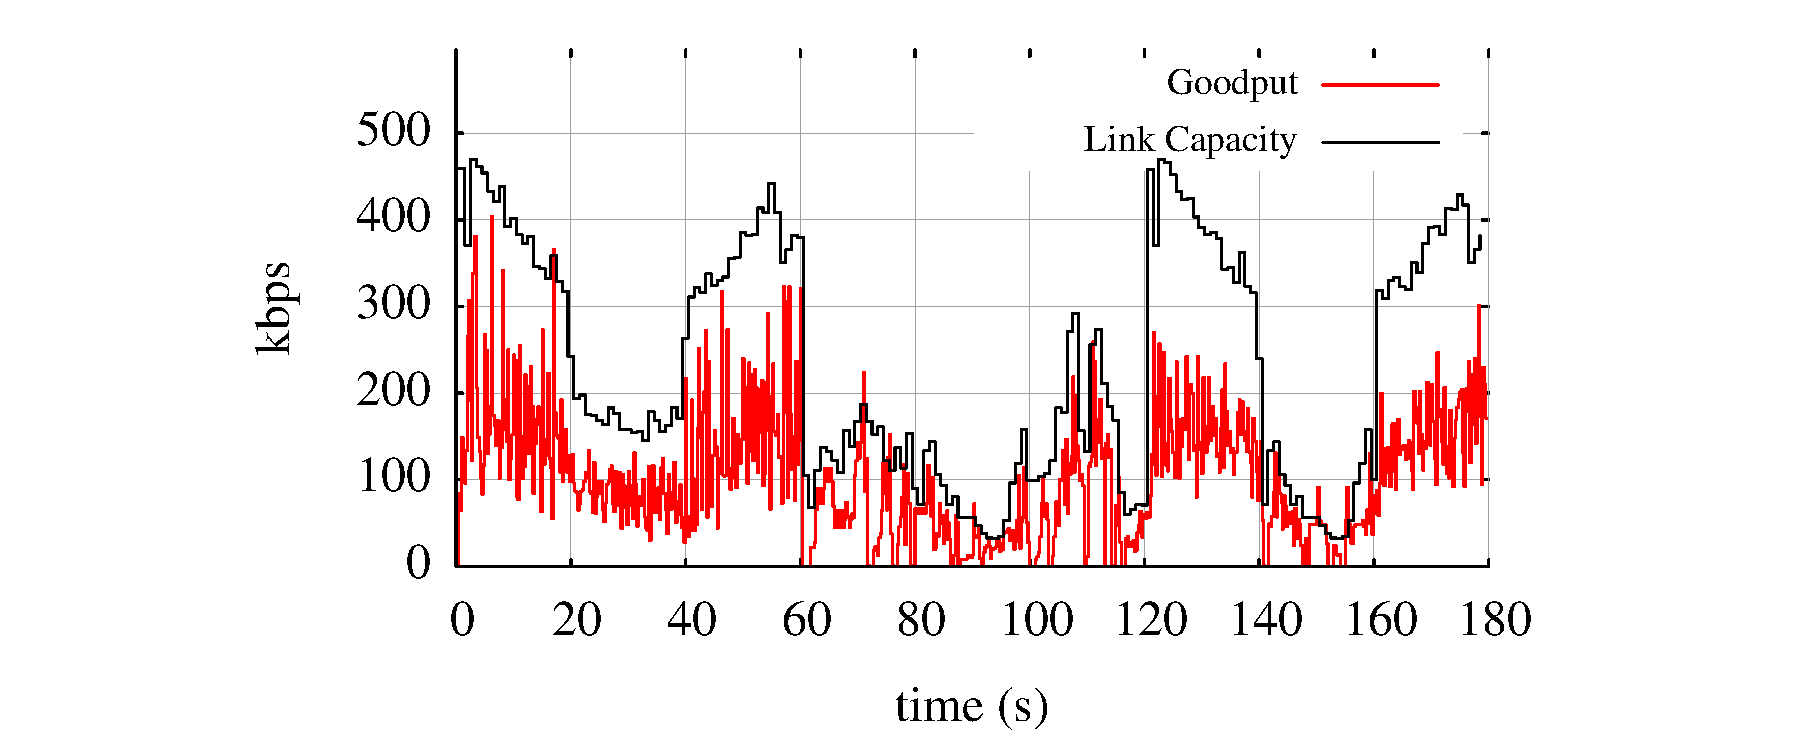
\includegraphics[width=0.5\textwidth, clip=true, trim=3cm 0 4.5cm 0]
      {chap8_graph_3g_tmmbr_b}
    }
  }
  \caption{Performance of bandwidth indications by the base stations in a slow
  time-varying link and 3G network.}
  \label{fig:tmmbn}
\end{figure}

\section{Out-of-path Congestion Cues}

Congestion Maps